Here's a scratch pad for all my results tables.

\section{2C19 MOE models}

\begin{table}[!h]
\begin{minipage}{.5\linewidth}
\centering
\begin{tabular}{|l|l|l|l|}
\hline
\multicolumn{4}{|c|}{2C19 Training Set Accuracy} \\ \hline
PC & Total          & Active          & Inactive \\ \hline
2  & 0.585          & 0.774           & 0.396   \\ \hline
5  & 0.685          & 0.726           & 0.645   \\ \hline
10 & 0.699          & 0.736           & 0.661    \\ \hline
15 & 0.700          & 0.747           & 0.653    \\ \hline
20 & 0.705          & 0.749           & 0.661    \\ \hline
30 & 0.717          & 0.761           & 0.672    \\ \hline
44 & 0.708          & 0.777           & 0.640    \\ \hline
\end{tabular}
\end{minipage}%
\begin{minipage}{.5\linewidth}
\centering
\begin{tabular}{|l|l|l|l|}
\hline
\multicolumn{4}{|c|}{2C19 Test Set Accuracy}       \\ \hline
PC & Total          & Active          & Inactive   \\ \hline
2  & 0.593          & 0.775           & 0.408      \\ \hline
5  & 0.683          & 0.729           & 0.635      \\ \hline
10 & 0.691          & 0.731           & 0.650      \\ \hline
15 & 0.687          & 0.736           & 0.637      \\ \hline
20 & 0.698          & 0.758           & 0.638      \\ \hline
30 & 0.699          & 0.764           & 0.633      \\ \hline
44 & 0.694          & 0.774           & 0.613      \\ \hline
\end{tabular}
\end{minipage}
\caption{2C19 MOE Model Accuracy}
%\caption{MOE model results 2C19 Test set}
\end{table}

Cytochrome P450 isozyme 2C19 models were trained on xxxxx of actives and xxxx of inactives in the training set, and validated against xxxx actives and xxxx inactives in the test set. All models are considered good models when the  total accuracy is above 0.6. Validating these models against the test set does not produce wildly divergent accuracy scores, indicating that overfitting is unlikely. The test set results represent compounds unseen by the model. 


\begin{figure}[!h]
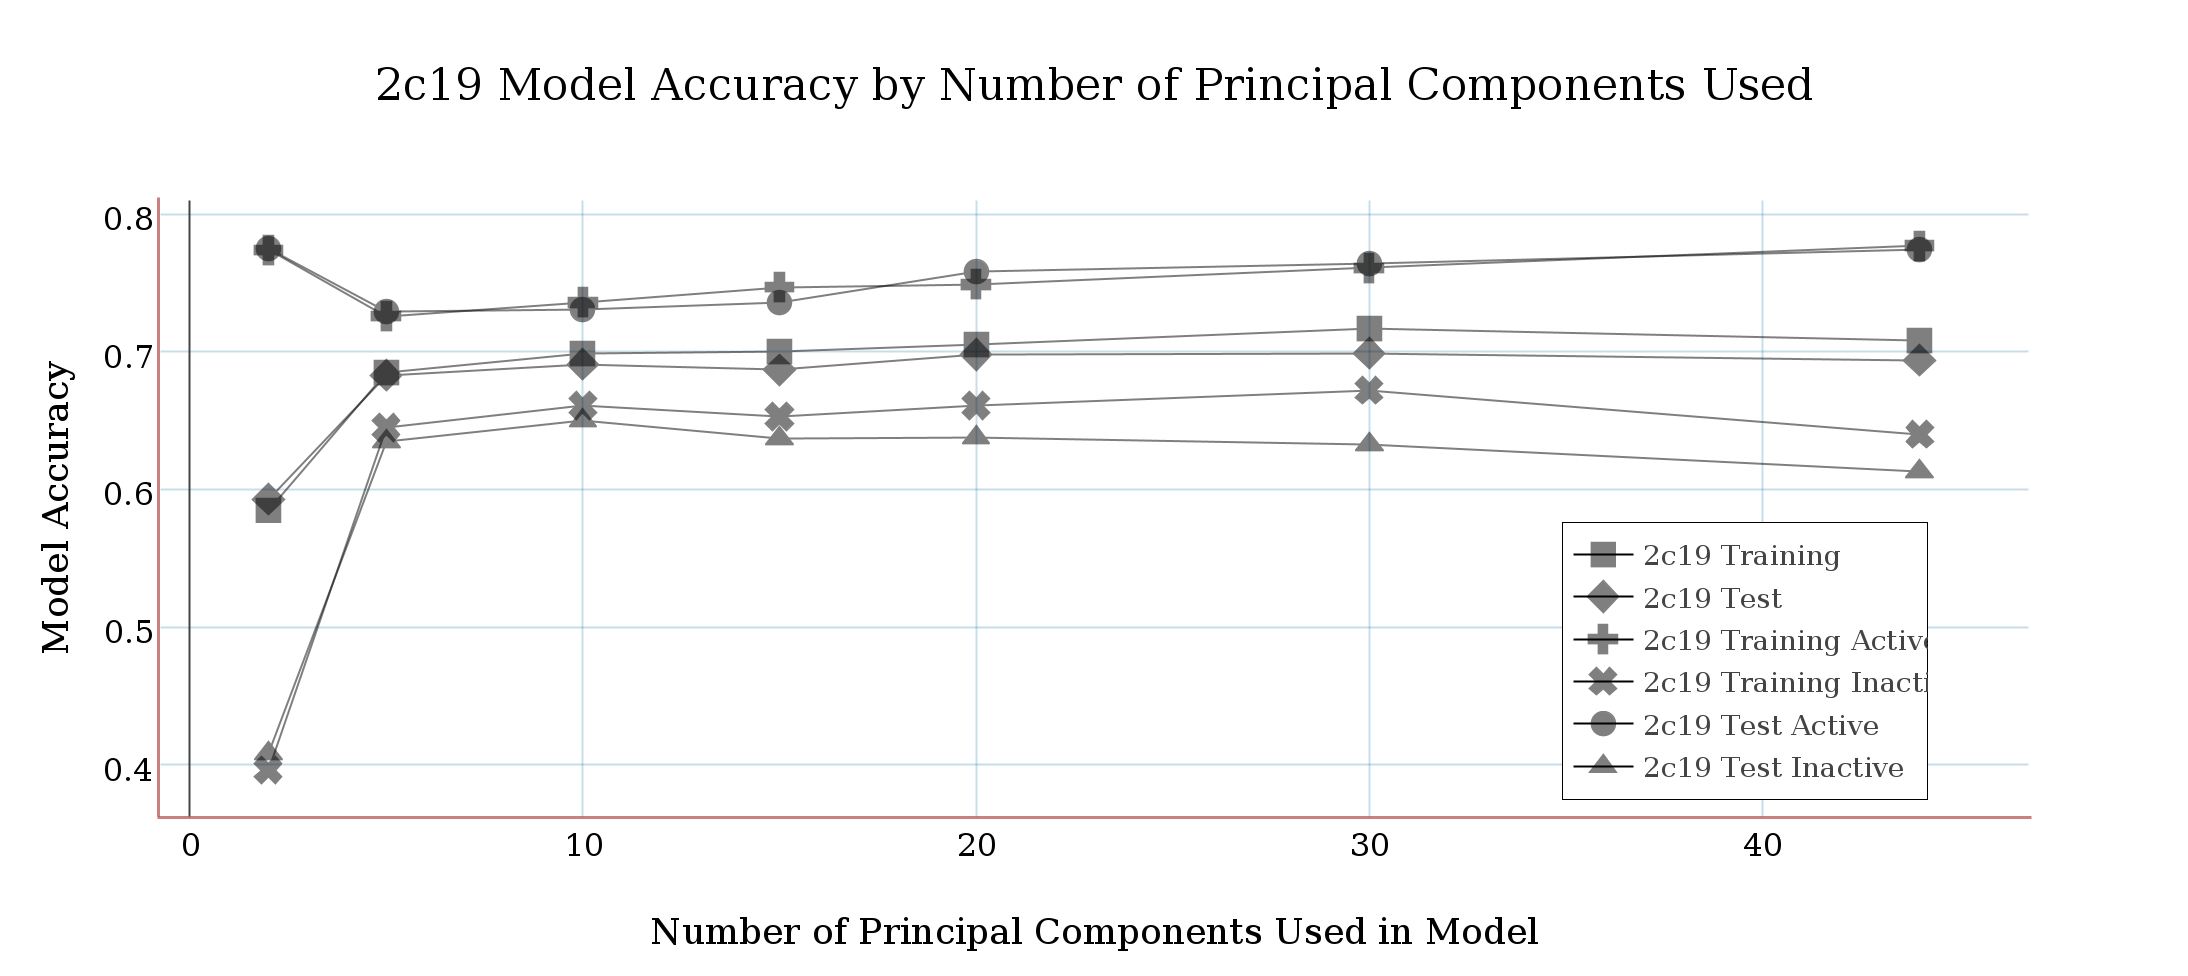
\includegraphics[width=1\textwidth]{../img/2c19_moe_model_accuracy.png}
\caption{2C19 MOE Model Accuracy}
\end{figure}

A visual scan of figure shows that model accuracy is higher for predicting active compounds than inactive compounds, and total accuracy is somewhere in between. 20 pricipal components (PC20) appears to be an optimal number for capturing relevant variance while minimizing Type II errors. At 20PCs, the total accuracy on the test set is 0.698. Accuracy on Actives is 0.758 and accuracy on inactives is 0.638.


\section{2C9 MOE Models}

\begin{table}[!h]
\begin{minipage}{.5\linewidth}
\centering
\begin{tabular}{|l|l|l|l|}
\hline
\multicolumn{4}{|c|}{2C9 Training Set Accuracy} \\ \hline
PC & Total          & Active          & Inactive\\ \hline
2  & 0.620          & 0.695           & 0.547   \\ \hline
5  & 0.683          & 0.722           & 0.645   \\ \hline
10 & 0.699          & 0.744           & 0.655   \\ \hline
15 & 0.702          & 0.752           & 0.653   \\ \hline
20 & 0.710          & 0.756           & 0.665   \\ \hline
30 & 0.711          & 0.754           & 0.668   \\ \hline
44 & 0.712          & 0.770           & 0.655   \\ \hline
\end{tabular}
\end{minipage}
\begin{minipage}{.5\linewidth}
\centering
\begin{tabular}{|l|l|l|l|}
\hline
\multicolumn{4}{|c|}{2C9 Test Set Accuracy}     \\ \hline
PC & Total          & Active          & Inactive\\ \hline
2  & 0.609          & 0.702           & 0.510   \\ \hline
5  & 0.675          & 0.713           & 0.634   \\ \hline
10 & 0.682          & 0.730           & 0.632   \\ \hline
15 & 0.686          & 0.739           & 0.630   \\ \hline
20 & 0.685          & 0.731           & 0.636   \\ \hline
30 & 0.690          & 0.730           & 0.646   \\ \hline
44 & 0.688          & 0.750           & 0.621   \\ \hline
\end{tabular}
\end{minipage}
\caption{2C9 MOE model results}
\end{table}

Cytochrome P450 isozyme 2C9 models were trained on xxxx of actives and xxxx of inactives in the training set, and validated against xxxx actives and xxxx inactives in the test set. All models are considered good models when the total accuracy is above 0.6. Validating these models against the test set does not produce wildly divergent accuracy scores, indicating that overfitting is unlikely. The test set results represent compounds unseen by the model. 

\begin{figure}[!h]
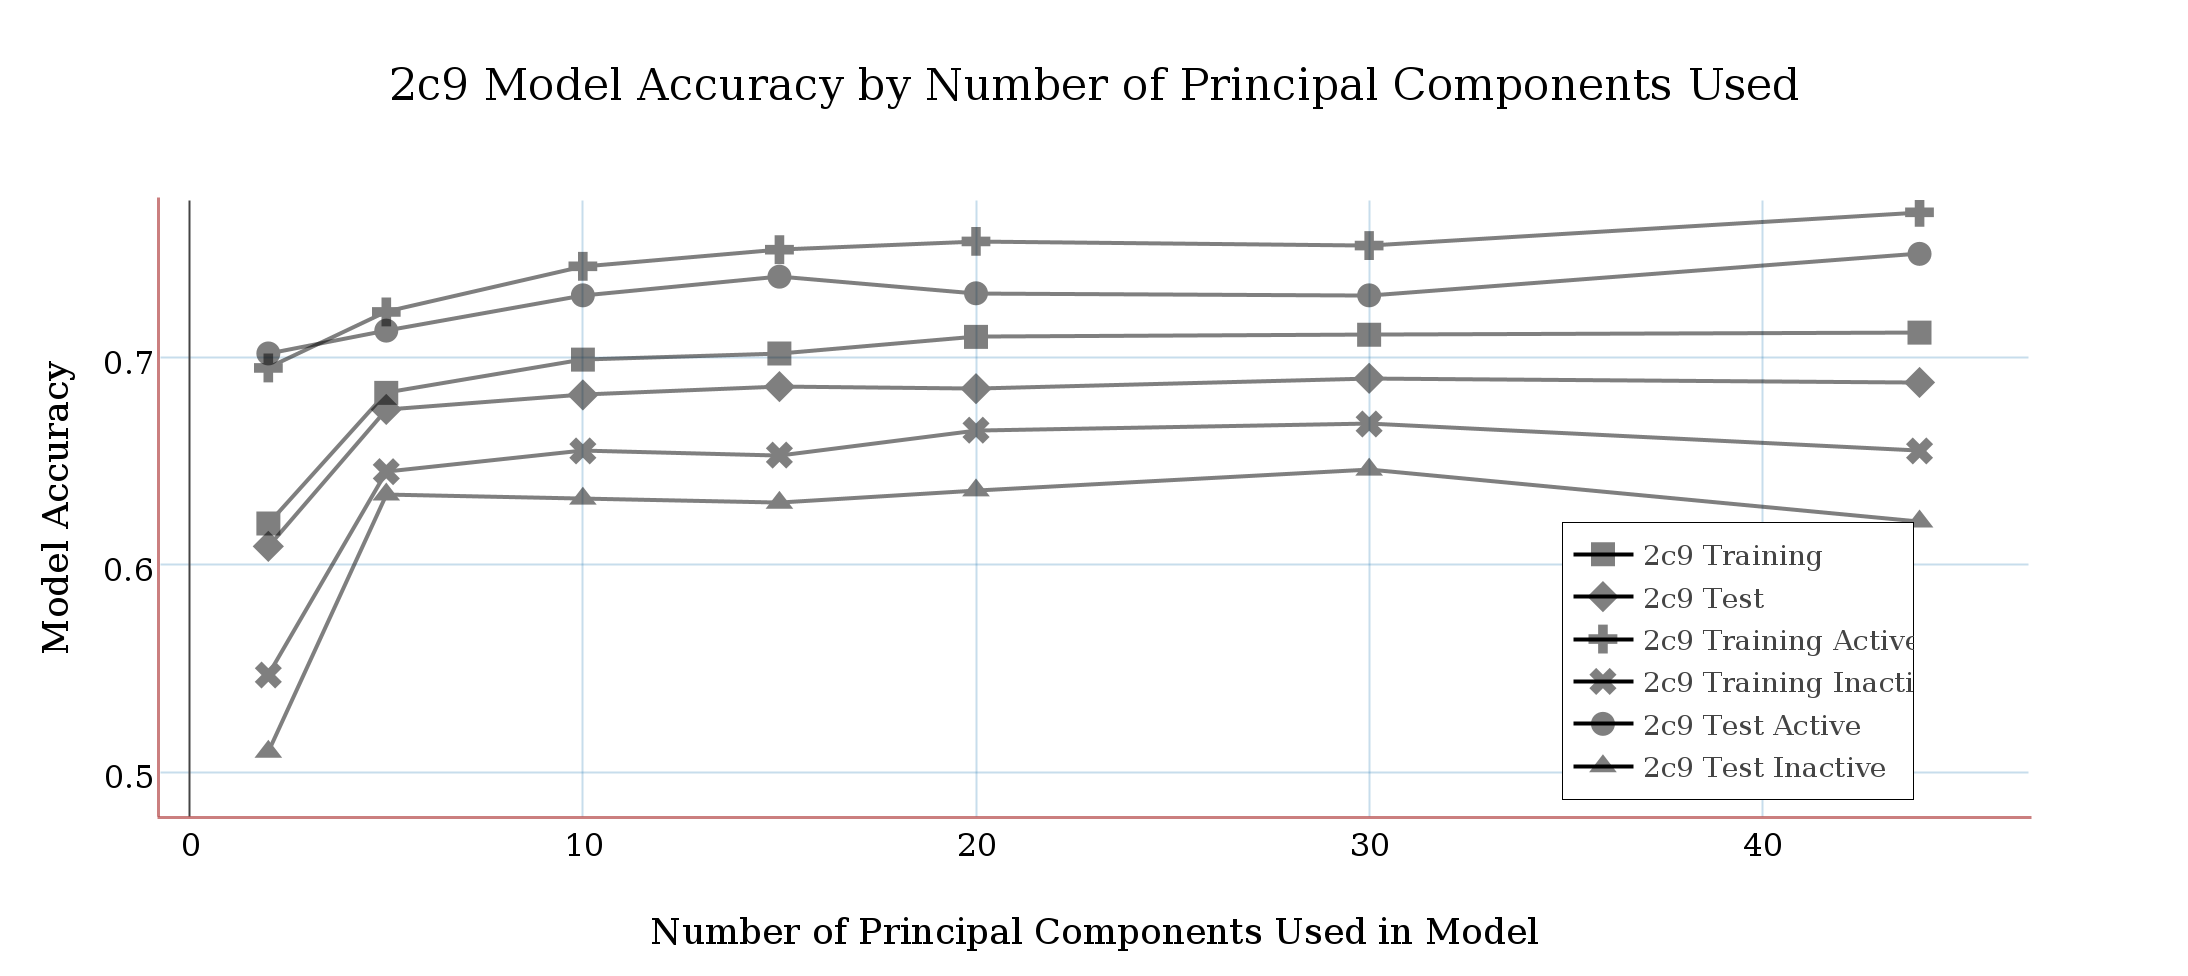
\includegraphics[width=1\textwidth]{../img/2c9_moe_model_accuracy.png}
\caption{2C19 MOE Model Accuracy}
\end{figure}

A visual scan of figure shows that model accuracy is higher for predicting active compounds than inactive compounds, and total accuracy is somewhere in between. 20 pricipal components (PC20) appears to be an optimal number for capturing relevant variance while minimizing Type II errors. At 20PCs, the total accuracy on the test set is 0.685. Accuracy on Actives is 0.731 and accuracy on inactives is 0.636.

\section{1A2 MOE Models}

\begin{table}[!h]
\begin{minipage}{.5\linewidth}
\centering
\begin{tabular}{|l|l|l|l|}
\hline
\multicolumn{4}{|c|}{1A2 Training Set Accuracy}   \\ \hline
PC & Total          & Active          & Inactive  \\ \hline
2  & 0.638          & 0.752           & 0.522     \\ \hline
5  & 0.704          & 0.746           & 0.662     \\ \hline
10 & 0.734          & 0.755           & 0.712     \\ \hline
15 & 0.737          & 0.770           & 0.704     \\ \hline
20 & 0.741          & 0.781           & 0.701     \\ \hline
30 & 0.735          & 0.782           & 0.686     \\ \hline
44 & 0.725          & 0.777           & 0.672     \\ \hline
\end{tabular}
\end{minipage}
\begin{minipage}{.5\linewidth}
\centering
\begin{tabular}{|l|l|l|l|}
\hline
\multicolumn{4}{|c|}{1A2 Test Set Accuracy}     \\ \hline
PC & Total          & Active          & Inactive \\ \hline
2  & 0.632          & 0.758           & 0.517   \\ \hline
5  & 0.705          & 0.773           & 0.643   \\ \hline
10 & 0.746          & 0.749           & 0.743   \\ \hline
15 & 0.752          & 0.775           & 0.731   \\ \hline
20 & 0.748          & 0.779           & 0.721   \\ \hline
30 & 0.739          & 0.783           & 0.698   \\ \hline
44 & 0.720          & 0.773           & 0.672   \\ \hline
\end{tabular}
\end{minipage}
\caption{1A2 MOE model results}
\end{table}

Cytochrome P450 isozyme 1A2 models were trained on xxxx of actives and xxxx of inactives in the training set, and validated against xxxx actives and xxxx inactives in the test set. All models are considered good models when the total accuracy is above 0.6. Validating these models against the test set does not produce wildly divergent accuracy scores, indicating that overfitting is unlikely. The test set results represent compounds unseen by the model. 

\begin{figure}[!h]
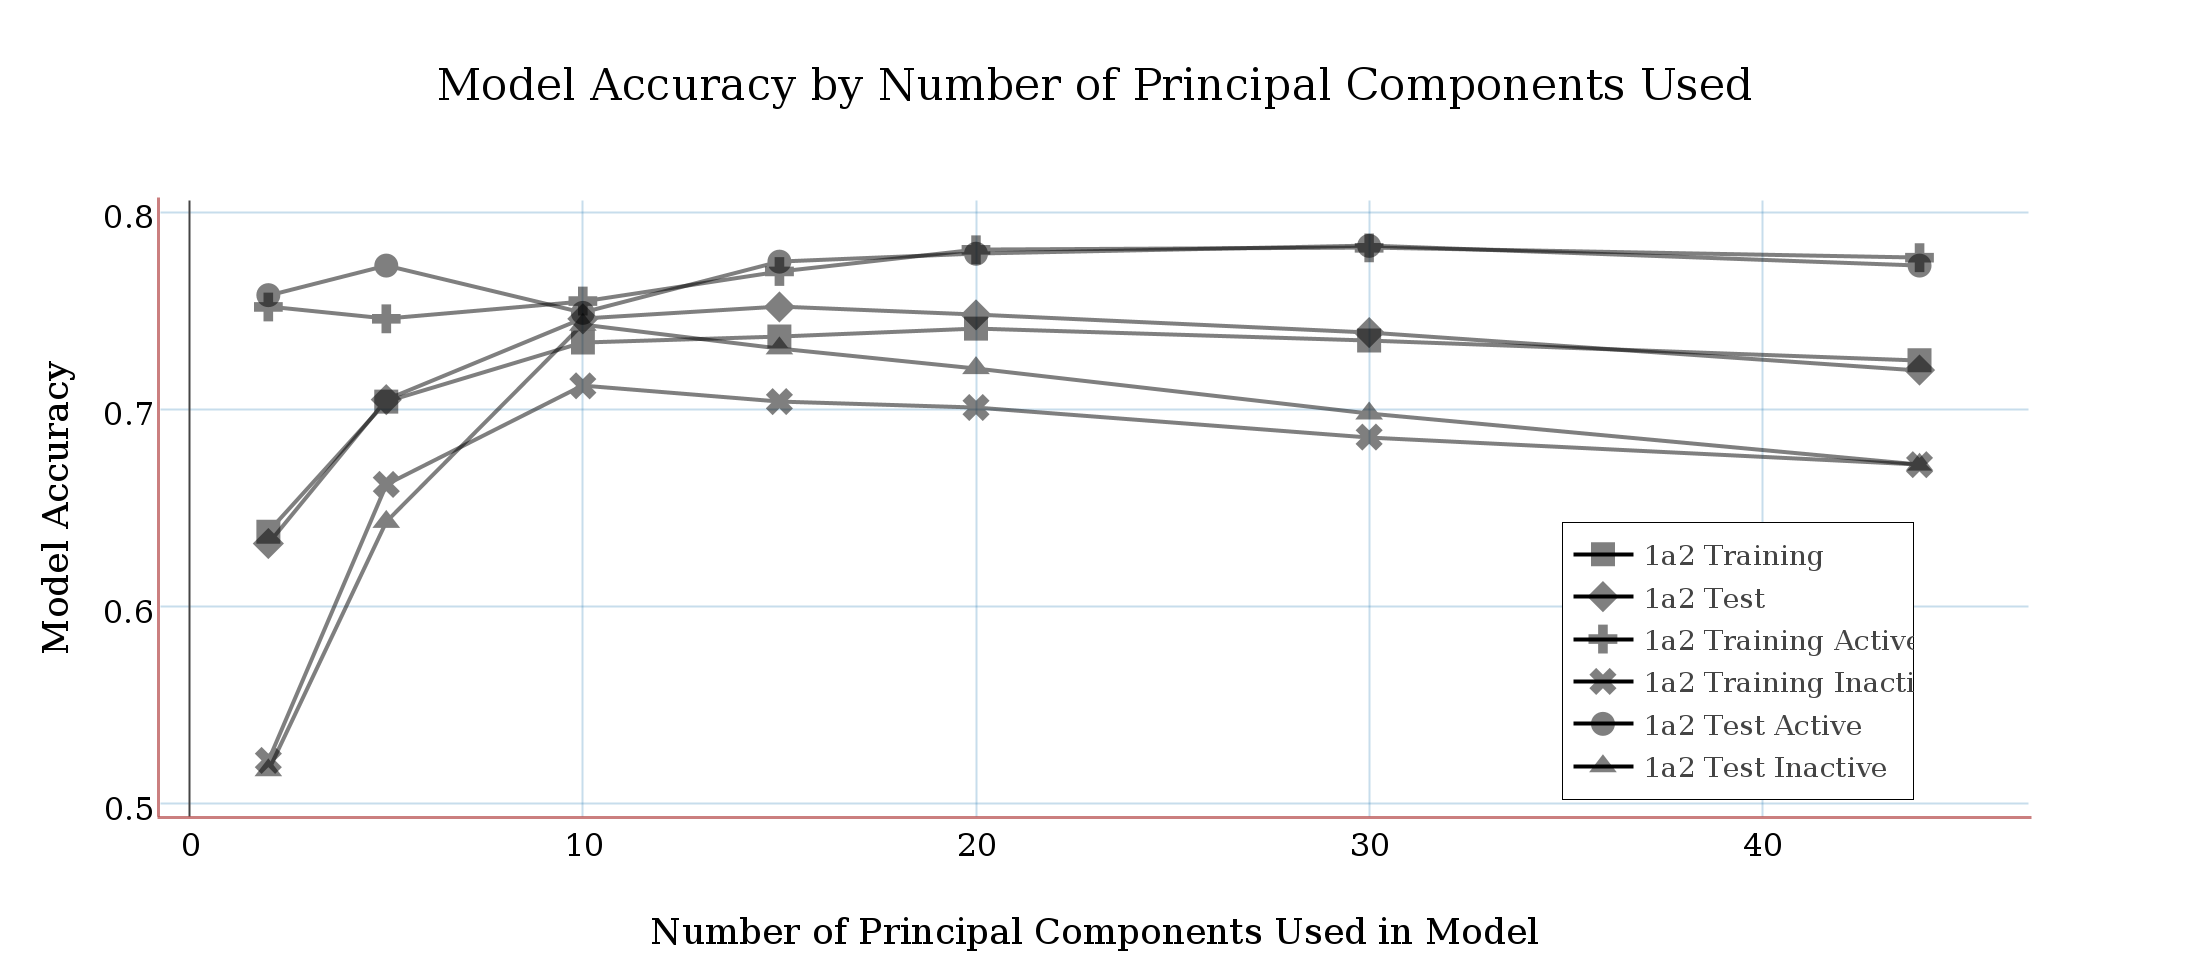
\includegraphics[width=1\textwidth]{../img/1a2_moe_model_accuracy.png}
\caption{1A2 MOE Model Accuracy}
\end{figure}

A visual scan of figure shows that model accuracy is higher for predicting active compounds than inactive compounds, and total accuracy is somewhere in between. 20 pricipal components (PC20) appears to be an optimal number for capturing relevant variance while minimizing Type II errors. At 20PCs, the total accuracy on the test set is 0.748. Accuracy on Actives is 0.779 and accuracy on inactives is 0.721.

\section{2D6 MOE Models}

\begin{table}[!h]
\begin{minipage}{.5\linewidth}
\centering
\begin{tabular}{|l|l|l|l|}
\hline
\multicolumn{4}{|c|}{2D6 Training Set Accuracy} \\ \hline
PC & Total          & Active          & Inactive\\ \hline
2  & 0.589          & 0.753           & 0.426   \\ \hline
5  & 0.670          & 0.706           & 0.634   \\ \hline
10 & 0.685          & 0.721           & 0.648   \\ \hline
15 & 0.686          & 0.709           & 0.662   \\ \hline
20 & 0.705          & 0.721           & 0.689   \\ \hline
30 & 0.703          & 0.732           & 0.673   \\ \hline
44 & 0.690          & 0.725           & 0.656   \\ \hline
\end{tabular}
\end{minipage}
\begin{minipage}{.5\linewidth}
\centering
\begin{tabular}{|l|l|l|l|}
\hline
\multicolumn{4}{|c|}{2D6 Test Set Accuracy}      \\ \hline
PC & Total          & Active          & Inactive \\ \hline
2  & 0.590          & 0.738           & 0.443    \\ \hline
5  & 0.667          & 0.685           & 0.650    \\ \hline
10 & 0.662          & 0.688           & 0.636    \\ \hline
15 & 0.665          & 0.692           & 0.639    \\ \hline
20 & 0.683          & 0.699           & 0.668    \\ \hline
30 & 0.686          & 0.696           & 0.677    \\ \hline
44 & 0.669          & 0.707           & 0.632    \\ \hline
\end{tabular}
\end{minipage}
\caption{2D6 MOE model results}
\end{table}

Cytochrome P450 isozyme 2D6 models were trained on xxxx of actives and xxxx of inactives in the training set, and validated against xxxx actives and xxxx inactives in the test set. All models are considered good models when the total accuracy is above 0.6. Validating these models against the test set does not produce wildly divergent accuracy scores, indicating that overfitting is unlikely. The test set results represent compounds unseen by the model. 

\begin{figure}[!h]
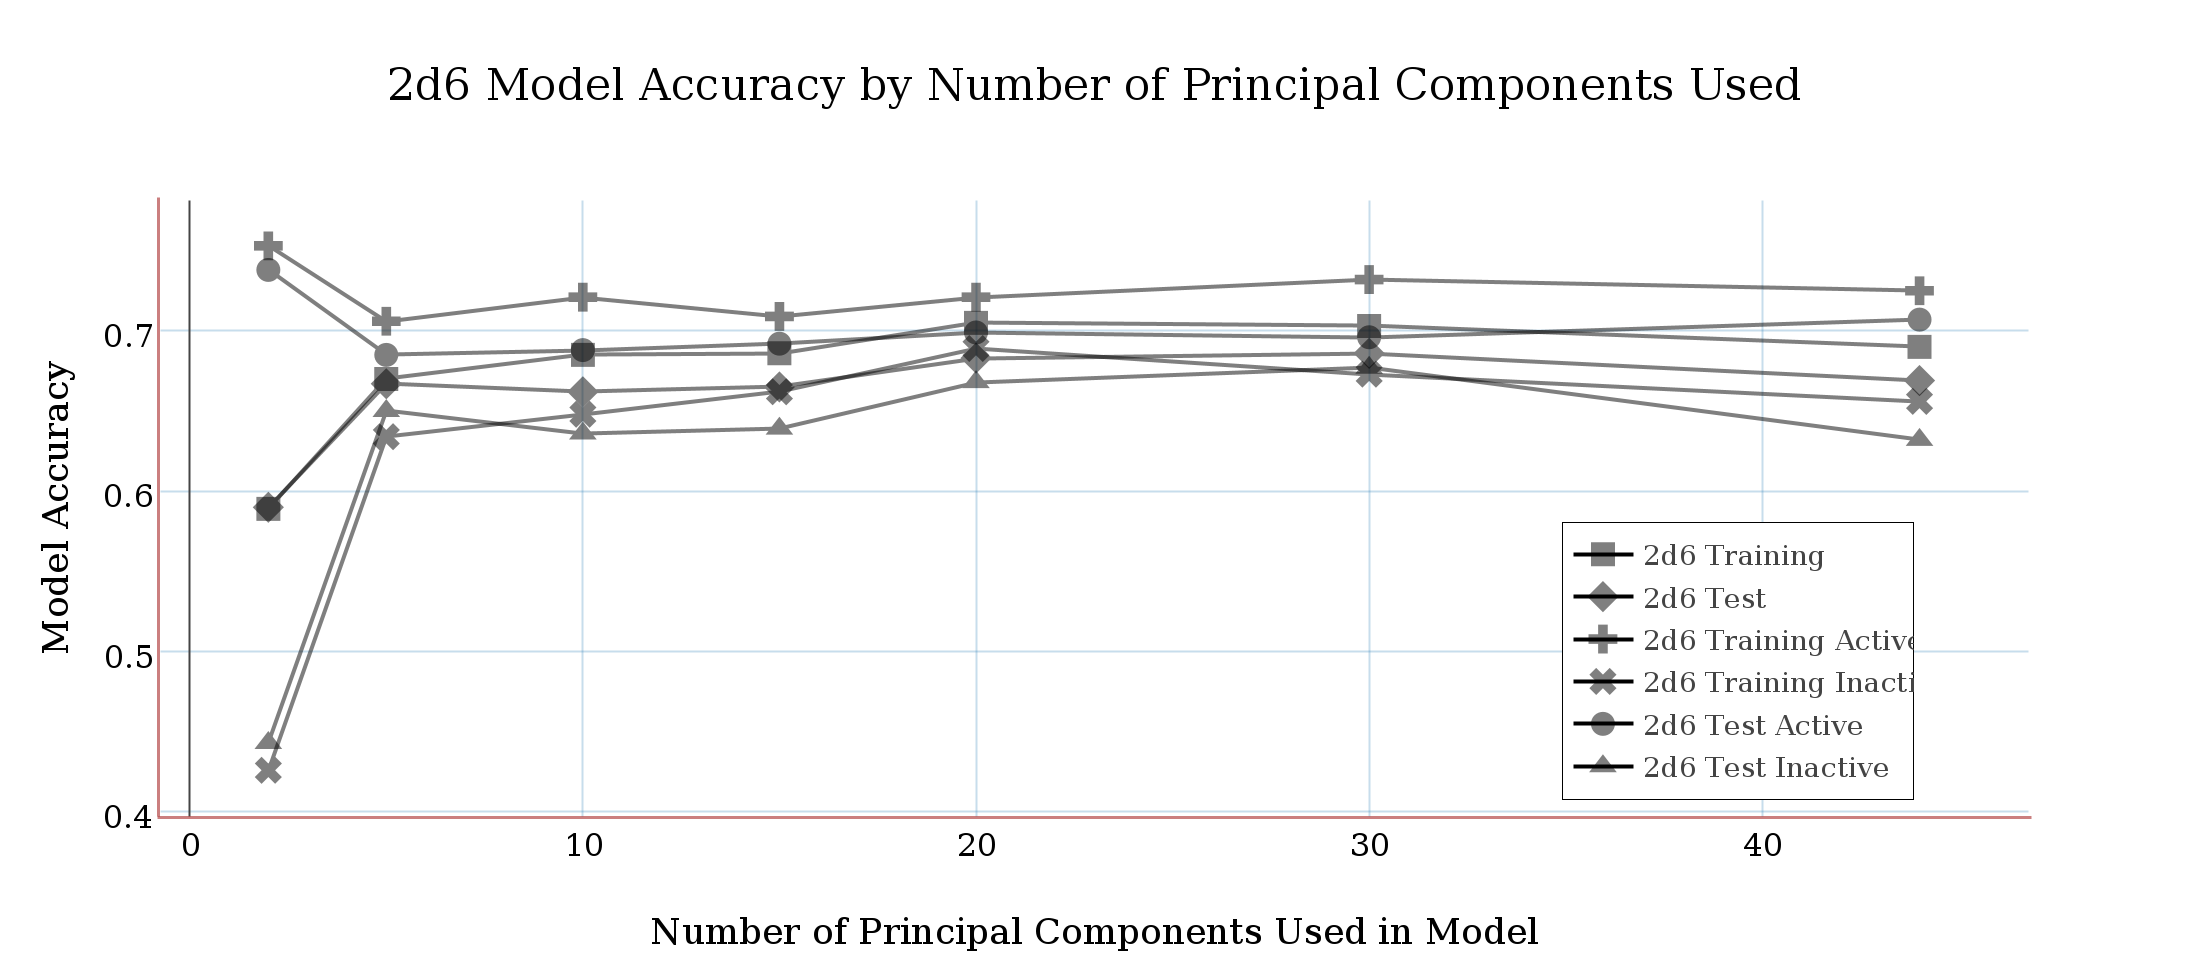
\includegraphics[width=1\textwidth]{../img/2d6_moe_model_accuracy.png}
\caption{2D6 MOE Model Accuracy}
\end{figure}

A visual scan of figure shows that model accuracy is higher for predicting active compounds than inactive compounds, and total accuracy is somewhere in between. 20 pricipal components (PC20) appears to be an optimal number for capturing relevant variance while minimizing Type II errors. At 20PCs, the total accuracy on the test set is 0.683. Accuracy on Actives is 0.699 and accuracy on inactives is 0.668.


\section{3A4 MOE Models}

\begin{table}[!h]
\begin{minipage}{.5\linewidth}
\centering
\begin{tabular}{|l|l|l|l|}
\hline
\multicolumn{4}{|c|}{3A4 Training Set Accuracy} \\ \hline
PC & Total          & Active          & Inactive \\ \hline
2  & 0.644          & 0.699           & 0.589   \\ \hline
5  & 0.675          & 0.727           & 0.623   \\ \hline
10 & 0.698          & 0.741           & 0.655   \\ \hline
15 & 0.701          & 0.746           & 0.656   \\ \hline
20 & 0.705          & 0.749           & 0.660   \\ \hline
30 & 0.709          & 0.761           & 0.657   \\ \hline
44 & 0.698          & 0.773           & 0.623   \\ \hline
\end{tabular}
\end{minipage}
\begin{minipage}{.5\linewidth}
\centering
\begin{tabular}{|l|l|l|l|}
\hline
\multicolumn{4}{|c|}{3A4 Test Set Accuracy}      \\ \hline
PC & Total          & Active          & Inactive \\ \hline
2  & 0.627          & 0.683           & 0.573    \\ \hline
5  & 0.656          & 0.719           & 0.595    \\ \hline
10 & 0.677          & 0.719           & 0.637    \\ \hline
15 & 0.680          & 0.733           & 0.628    \\ \hline
20 & 0.686          & 0.736           & 0.638    \\ \hline
30 & 0.686          & 0.742           & 0.631    \\ \hline
44 & 0.676          & 0.747           & 0.607    \\ \hline
\end{tabular}
\end{minipage}
\caption{3A4 MOE model results}
\end{table}

Cytochrome P450 isozyme 3A4 models were trained on xxxx of actives and xxxx of inactives in the training set, and validated against xxxx actives and xxxx inactives in the test set. All models are considered good models when the  total accuracy is above 0.6. Validating these models against the test set does not produce wildly divergent accuracy scores, indicating that overfitting is unlikely. The test set results represent compounds unseen by the model. 

\begin{figure}[!h]
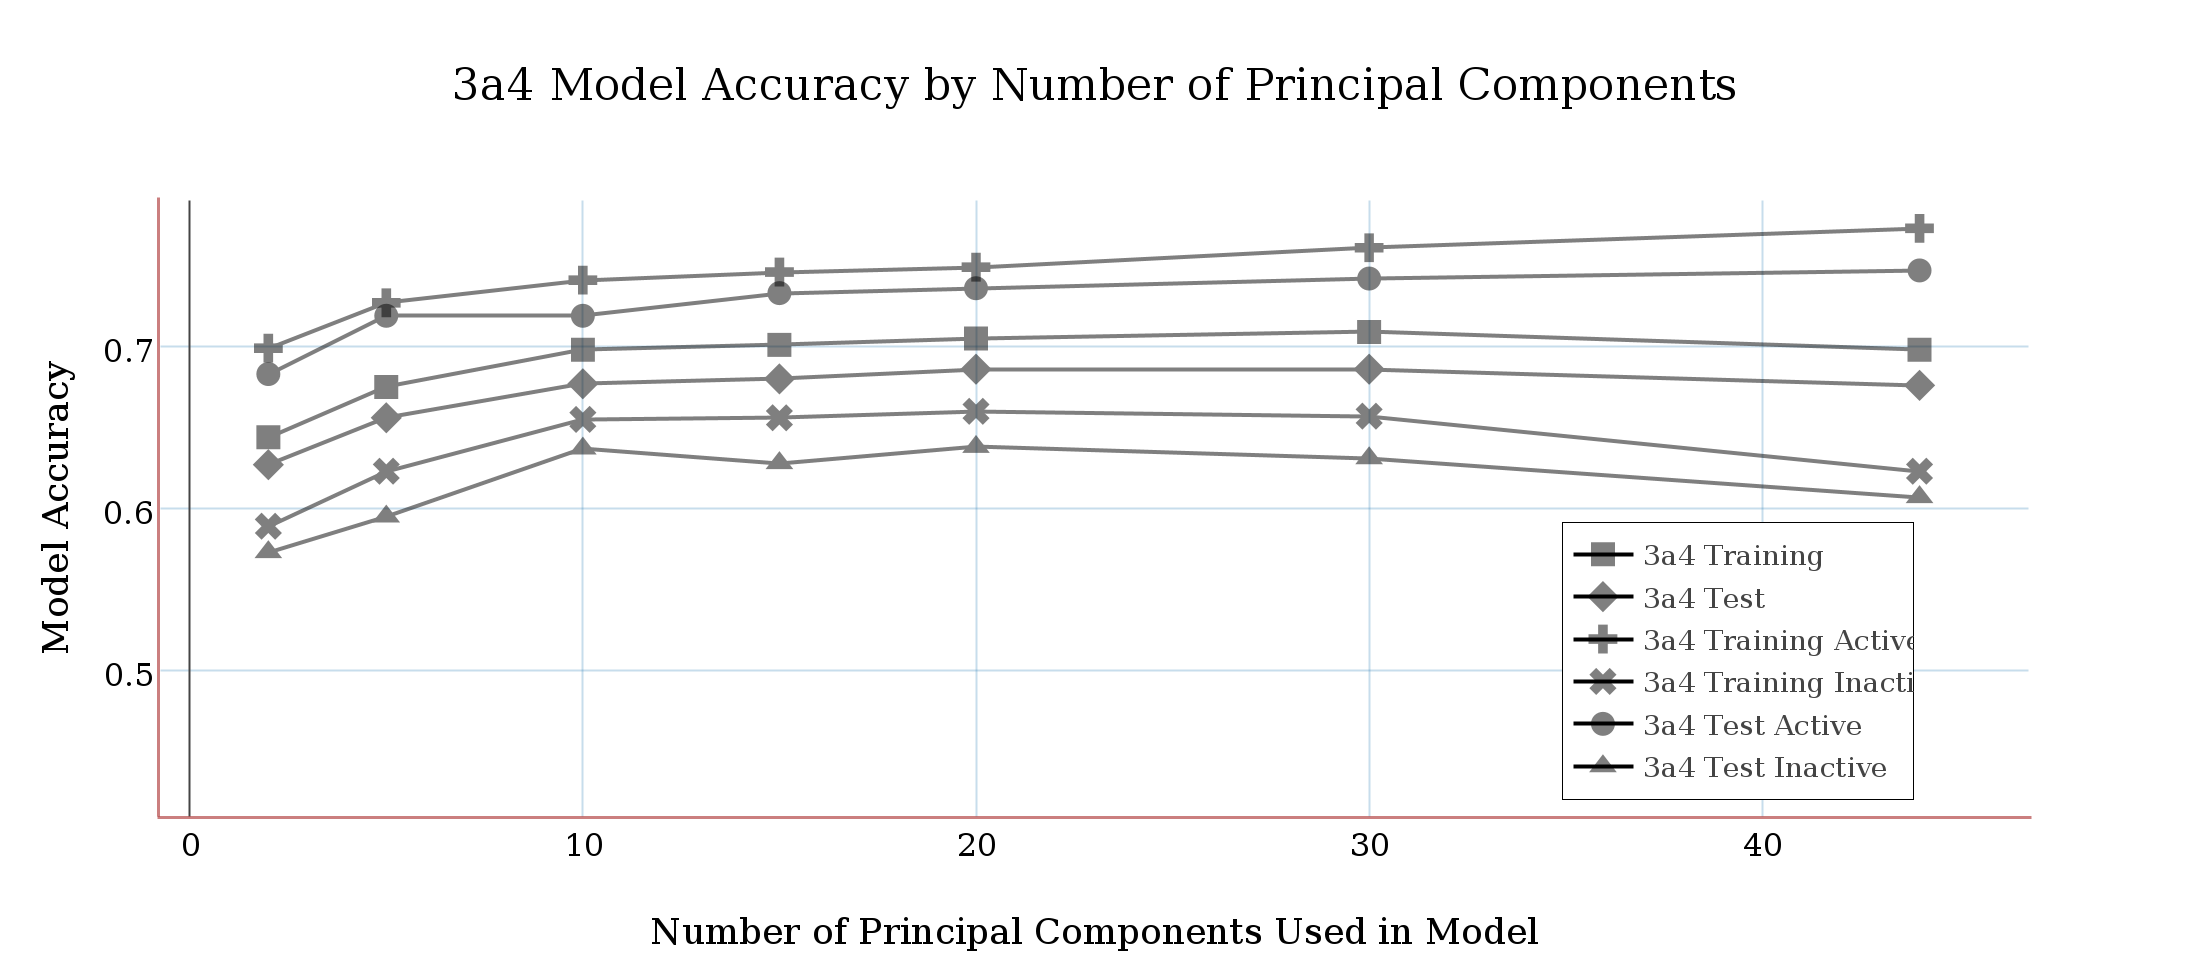
\includegraphics[width=1\textwidth]{../img/3a4_moe_model_accuracy.png}
\caption{3A4 MOE Model Accuracy}
\end{figure}

A visual scan of figure shows that model accuracy is higher for predicting active compounds than inactive compounds, and total accuracy is somewhere in between. 20 pricipal components (PC20) appears to be an optimal number for capturing relevant variance while minimizing Type II errors. At 20PCs, the total accuracy on the test set is 0.686. Accuracy on Actives is 0.736 and accuracy on inactives is 0.638.

\section{Comparison of Methods}
%%%
%\begin{table}[!h]
%\begin{tabular}{|l|l|l|l|l|l|}
%\hline
%\multicolumn{6}{|c|}{Training Set Methods Comparison} \\ \hline
%Isozyme       & 1A2   & 2C9   & 2C19  & 2D6   & 3A4   \\ \hline
%MOE 20pc      & 0.741 & 0.710 & 0.705 & 0.705 & 0.705 \\ \hline
%kNN           & 0.761 & 0.721 & 0.730 & 0.717 & 0.716 \\ \hline
%Random Forest & 0.770 & 0.717 & 0.736 & 0.729 & 0.719 \\ \hline
%SVD           & 0.800 & 0.749 & 0.767 & 0.755 & 0.755 \\ \hline
%Ensemble      &       &       &       &       &       \\ \hline
%\end{tabular}
%\caption{Comparison of methods for Training Set}
%\end{table}


\begin{figure}[!h]
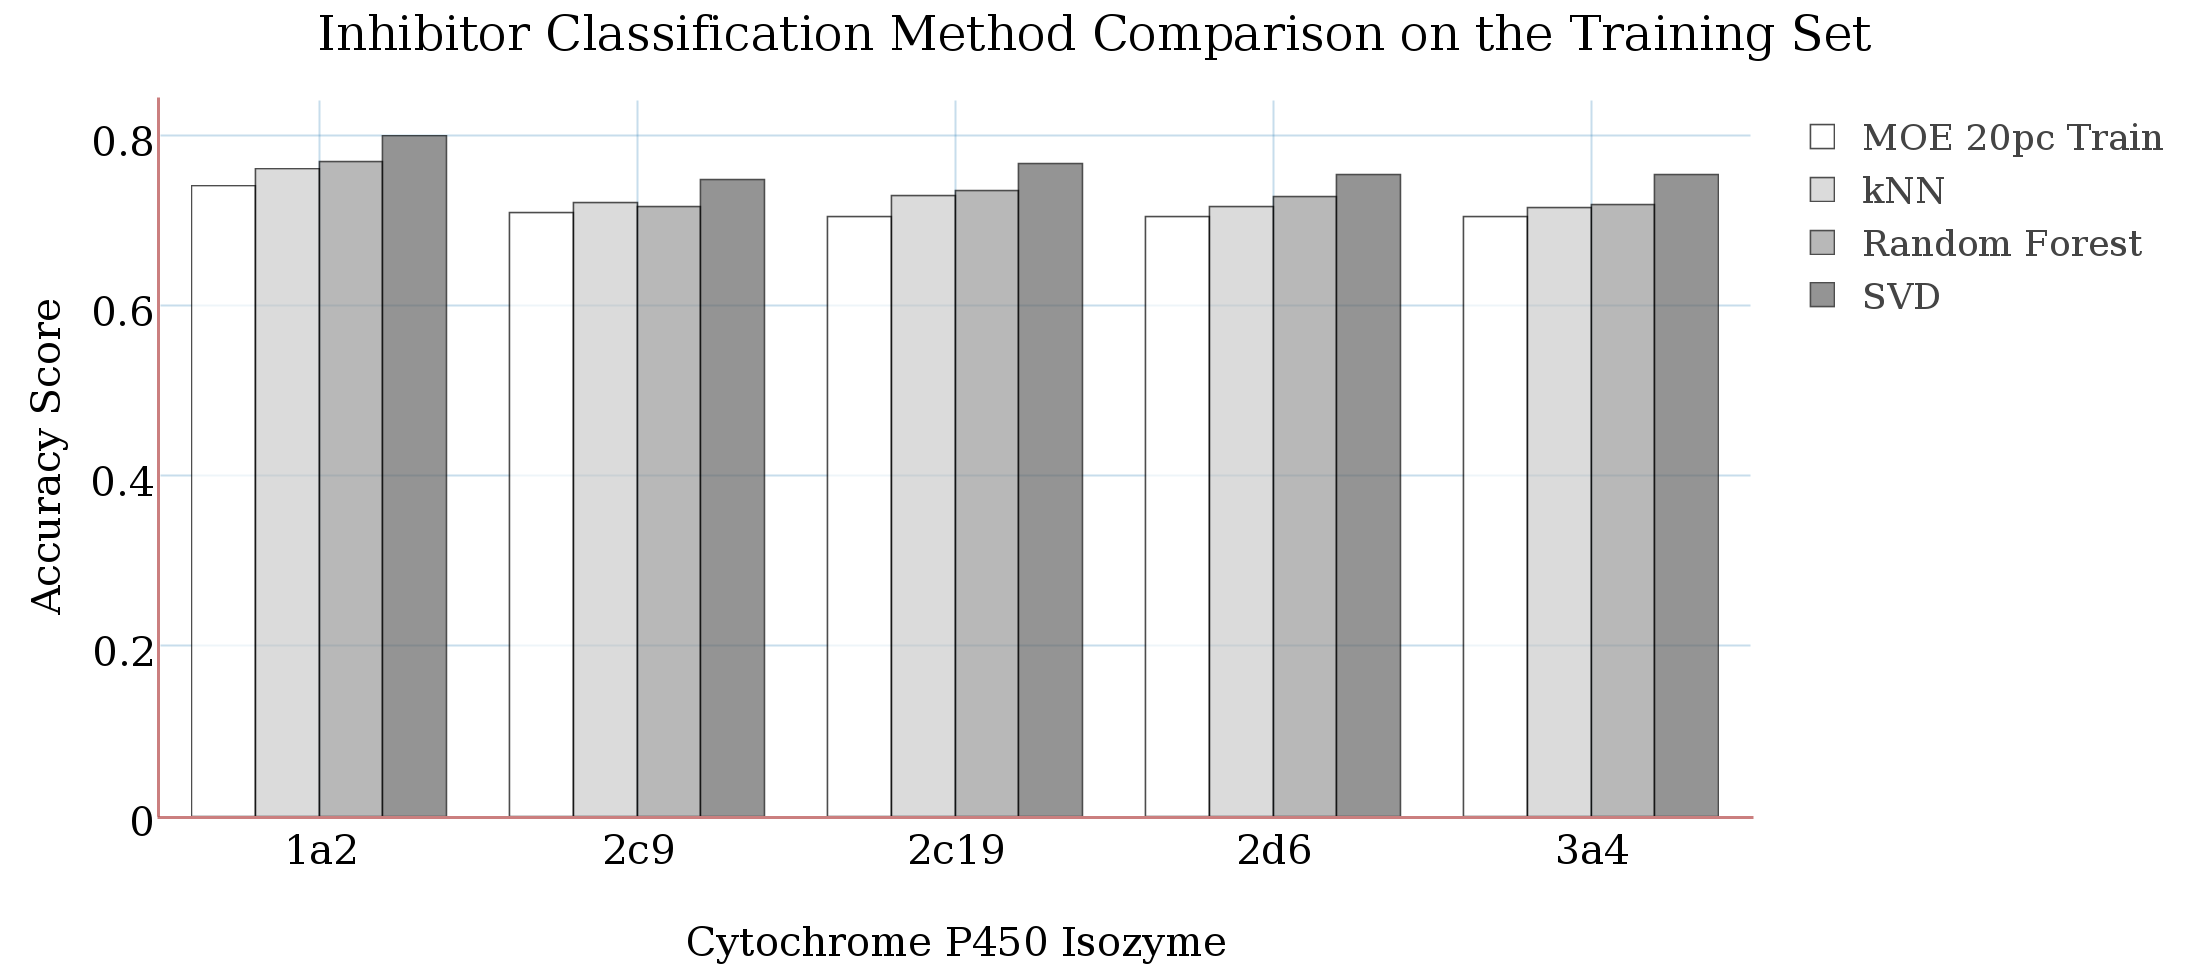
\includegraphics[width=1\textwidth]{../img/method_comparison_training_set.png}
\caption{Inhibitor Classification Method Comparison on the Training Set}
\end{figure}

\subsection{1A2}

\begin{table}[h]
\begin{tabular}{|l|l|l|}
\hline
\multicolumn{3}{|c|}{1A2 Classification Method Comparison} \\ \hline
          & Training Set & Test Set \\ \hline
MOE 20PC  & 0.741        & 0.748    \\ \hline
kNN       & 0.761        & 0.754    \\ \hline
Random Forest & 0.770    & 0.769    \\ \hline
SVD       & 0.800        & 0.804    \\ \hline
\end{tabular}
\caption{Comparison of Classification Methods for 1A2}
\end{table}

\subsection{2C9}

\begin{table}[h]
\begin{tabular}{|l|l|l|}
\hline
\multicolumn{3}{|c|}{2C9 Classification Method Comparison} \\ \hline
          & Training Set & Test Set \\ \hline
MOE 20PC  & 0.710        & 0.685    \\ \hline
kNN       & 0.721        & 0.692    \\ \hline
Random Forest & 0.717    & 0.687    \\ \hline
SVD       & 0.749        & 0.720    \\ \hline
\end{tabular}
\caption{Comparison of Classification Methods for 2C9}
\end{table}

\subsection{2C19}

\begin{table}[h]
\begin{tabular}{|l|l|l|}
\hline
\multicolumn{3}{|c|}{2C19 Classification Method Comparison} \\ \hline
          & Training Set & Test Set \\ \hline
MOE 20PC  & 0.705        & 0.698    \\ \hline
kNN       & 0.730        & 0.720    \\ \hline
Random Forest & 0.736    & 0.721    \\ \hline
SVD       & 0.767        & 0.756    \\ \hline
\end{tabular}
\caption{Comparison of Classification Methods for 2C19}
\end{table}

\subsection{2D6}

\begin{table}[h]
\begin{tabular}{|l|l|l|}
\hline
\multicolumn{3}{|c|}{2D6 Classification Method Comparison} \\ \hline
          & Training Set & Test Set \\ \hline
MOE 20PC  & 0.705        & 0.683    \\ \hline
kNN       & 0.717        & 0.678    \\ \hline
Random Forest & 0.729    & 0.707    \\ \hline
SVD       & 0.755        & 0.725    \\ \hline
\end{tabular}
\caption{Comparison of Classification Methods for 2D6}
\end{table}

\subsection{3A4}

\begin{table}[h]
\begin{tabular}{|l|l|l|}
\hline
\multicolumn{3}{|c|}{3A4 Classification Method Comparison} \\ \hline
          & Training Set & Test Set \\ \hline
MOE 20PC  & 0.705        & 0.686    \\ \hline
kNN       & 0.716        & 0.674    \\ \hline
Random Forest & 0.719    & 0.683    \\ \hline
SVD       & 0.755        & 0.714    \\ \hline
\end{tabular}
\caption{Comparison of Classification Methods for 3A4}
\end{table}

%\begin{table}[!h]
%\begin{tabular}{|l|l|l|l|l|l|}
%\hline
%\multicolumn{6}{|c|}{Test Set Methods Comparison}     \\ \hline
%Isozyme       & 1A2   & 2C9   & 2C19  & 2D6   & 3A4   \\ \hline
%MOE 20pc      & 0.748 & 0.685 & 0.698 & 0.683 & 0.686 \\ \hline
%kNN           & 0.754 & 0.692 & 0.720 & 0.678 & 0.674 \\ \hline
%Random Forest & 0.769 & 0.687 & 0.721 & 0.707 & 0.683 \\ \hline
%SVD           & 0.804 & 0.720 & 0.756 & 0.725 & 0.714 \\ \hline
%Ensemble      &       &       &       &       &       \\ \hline
%\end{tabular}
%\caption{Comparison of Methods for Test Sets}
%\end{table}

\begin{figure}[!h]
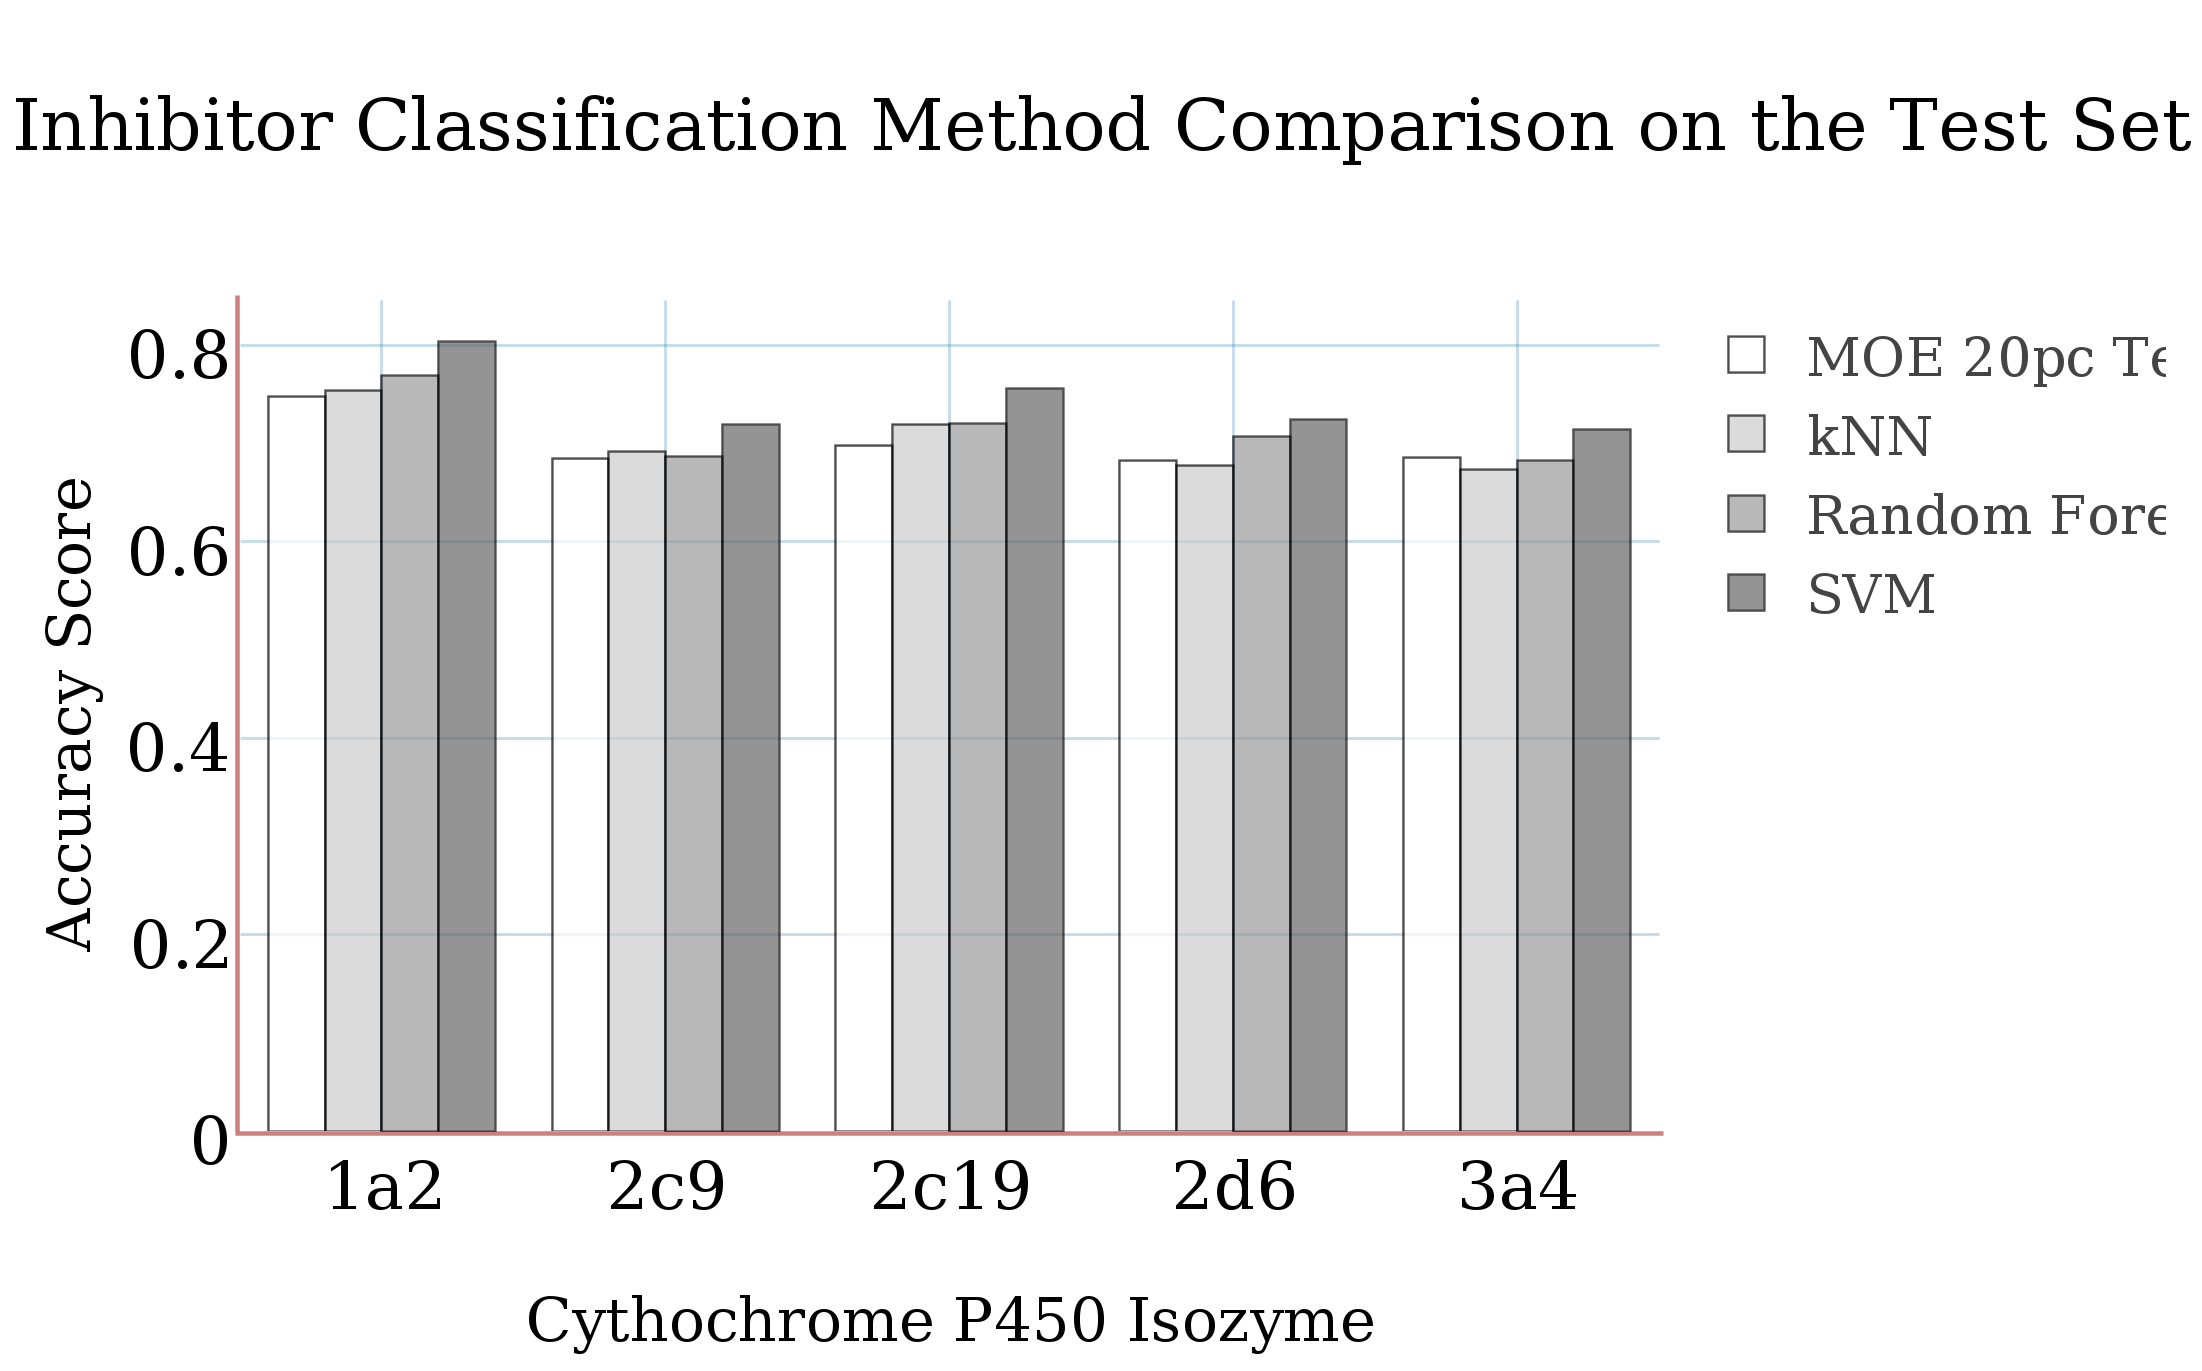
\includegraphics[width=1\textwidth]{../img/method_comparison_test_set.png}
\caption{Inhibitor Classification Method Comparison on the Test Set}
\end{figure}






